\documentclass{Z}

%% need no \usepackage{Sweave}
\usepackage{thumbpdf}

%% new commands
\newcommand{\class}[1]{``\code{#1}''}
\newcommand{\fct}[1]{\code{#1()}}

\author{Achim Zeileis\\Wirtschaftsuniversit\"at Wien \And
        Christian Kleiber\\Universit\"at Basel \And
	Simon Jackman\\Stanford University}
\Plainauthor{Achim Zeileis, Christian Kleiber, Simon Jackman}

\title{Regression Models for Count Data in \proglang{R}}
\Plaintitle{Regression Models for Count Data in R}

\Keywords{GLM, Poisson model, negative binomial model, zero-inflated model, hurdle model}

\Abstract{
  The classical Poisson, geometric and negative binomial regression models 
  for count data belong to the family of generalized linear models and
  are available at the core of the statistics toolbox in the \proglang{R}
  system for statistical computing. After reviewing the conceptual and
  computational features of these methods, a new implementation of
  zero-inflated and hurdle regression models in the functions \fct{zeroinfl}
  and \fct{hurdle} from the package \pkg{pscl} is introduced. It re-uses
  design and functionality of the basic \proglang{R} functions just
  as the underlying conceptual tools extend the classical models.
  Both zero-inflated and hurdle models, are able to incorporate over-dispersion and
  excess zeros---two problems
  that typically occur in count data sets in economics and the social
  sciences---better than their classical counterparts.
  Using cross-section data on the demand for medical care, it is illustrated
  how the classical as well as the zero-augmented models can be fitted,
  inspected and tested in practice.
}

\begin{document}


%\VignetteIndexEntry{Regression Models for Count Data in R}
%\VignetteDepends{sandwich,zoo,lmtest,MASS,car}
%\VignetteKeywords{GLM, Poisson model, negative binomial model, zero-inflated model, hurdle model}
%\VignettePackage{pscl}


\section{Introduction} \label{sec:intro}

Modeling count variables is a common task in economics and the social
sciences. The classical Poisson regression model for count
data is often of limited use in these disciplines because empirical
count data sets typically exhibit over-dispersion and/or an excess
number of zeros. The former issue can be addressed by extending 
the plain Poisson regression model in various directions: e.g.,
using sandwich covariances or estimating an additional dispersion
parameter (in a so-called quasi-Poisson model). Another more formal
way is to use a negative binomial (NB) regression. All of these models
belong to the family of generalized linear models 
\citep[GLMs, see][]{countreg:Nelder+Wedderburn:1972,countreg:McCullagh+Nelder:1989}.
However, although these models typically can capture over-dispersion
rather well, they are in many applications not sufficient for 
modeling excess zeros. Since \cite{countreg:Mullahy:1986} and
\cite{countreg:Lambert:1992} there is increased interest, both in the
statistics and econometrics literature, in zero-augmented models
that address this issue by a second model component capturing zero counts.
Zero-inflation models \citep{countreg:Lambert:1992}
are mixture models that combine a count component and a point mass at zero.
Hurdle models \citep{countreg:Mullahy:1986} take a somewhat different
approach and combine a left-truncated count component with a
right-censored hurdle component.
An overview of count data models in econometrics, including 
zero-inflated and hurdle models, is provided in
\cite{countreg:Cameron+Trivedi:1998,countreg:Cameron+Trivedi:2005}.

In \proglang{R} \citep{countreg:R:2007}, GLMs are provided
by the model fitting functions \fct{glm} \citep{countreg:Chambers+Hastie:1992}
in the \pkg{stats} package and \fct{glm.nb} in the \pkg{MASS}
package \citep{countreg:Venables+Ripley:2002} along with associated
methods for diagnostics and inference. Here, we discuss the implementation
of zero-inflated and hurdle models in the functions \fct{zeroinfl}
and \fct{hurdle} in the \pkg{pscl} package \citep{countreg:Jackman:2007},
available from the Comprehensive \proglang{R} Archive Network (CRAN)
at \url{http://CRAN.R-project.org/}.
The design of both modeling functions as well as the methods operating
on the associated fitted model objects follows that of the base \proglang{R}
functionality so that the new software integrates easily into the
computational toolbox for modeling count data in \proglang{R}.

The remainder of this paper is organized as follows: Section~\ref{sec:software}
discusses both the classical and zero-augmented count data models and their
\proglang{R} implementations. In Section~\ref{sec:illustrations}, all
count regression models discussed are applied to a microeconometric
cross-section data set on the demand for medical care. The summary in
Section~\ref{sec:summary} concludes the main part of the paper; further
technical details are presented in the appendix.


\section{Models and software} \label{sec:software}

In this section, we briefly outline the theory and its implementation in 
\proglang{R} \citep{countreg:R:2007} for some basic count data regression
models as well as their zero-augmented extensions (see Table~\ref{tab:overview}
for an overview). The classical Poisson, geometric
and negative binomial models are described in a generalized linear model (GLM)
framework; they are implemented in \proglang{R} by the \fct{glm} function
\citep{countreg:Chambers+Hastie:1992} in the \pkg{stats} package and the
\fct{glm.nb} function in the \pkg{MASS} package \citep{countreg:Venables+Ripley:2002}.
The zero-inflated and hurdle extensions of these models are provided by the
functions \fct{zeroinfl} and \fct{hurdle} in package \pkg{pscl} \citep{countreg:Jackman:2007}.
The original implementation of \cite{countreg:Jackman:2007} was improved
by \cite{countreg:Kleiber+Zeileis:2008} for \pkg{pscl} to make the fitting functions and the
fitted model objects more similar to their \fct{glm} and \fct{glm.nb} counterparts.
The most important features of the new \fct{zeroinfl} and \fct{hurdle} functions
are discussed below while some technical aspects are deferred to the appendix.
An alternative implementation of zero-inflated count models is available in
the function \fct{zicounts} from package \pkg{zicounts} \citep{countreg:Mwalili:2006}.
Additionally, it provides censored versions of classical and zero-inflated count
regression models. Another extension of zero-inflated Poisson models is available
in package \pkg{ZIGP} \citep{countreg:Erhardt:2007} which allows dispersion---in addition to
mean and zero-inflation level---to depend on regressors.
However, the interfaces of both packages are less standard with fewer (or no)
standard methods provided. Therefore, 
re-using generic inference tools is more cumbersome and hence these packages are
not discussed here. 


In addition to zero-augmented models, there are many further extensions to
the classical Poisson model which are not discussed here. Some important model
classes include mixed-effects models---available in \proglang{R} in packages
\pkg{lme4} and \pkg{nlme} \citep[see][]{countreg:Pinheiro+Bates:2000}---and
finite mixture models---implemented in \proglang{R} in package \pkg{flexmix}
\citep{countreg:Leisch:2004}---or generalized estimating equations
(GEE)---provided in \proglang{R} by package \pkg{geepack}
\citep{countreg:Halekoh+Hojsgaard+Yan:2006}. Further information about the models
and alternative \proglang{R} implementations can be found in the respective
references.

\begin{table}[b!]
\begin{center}
\begin{tabular}{|l|l|l|p{7.4cm}|}
\hline
Type & Distribution & Method & Description \\ \hline
GLM & Poisson & ML & Poisson regression (classical GLM, estimated by ML) \\
    &         & quasi & quasi-Poisson regression
                        (same mean function, estimated by quasi-ML/GEE,
			 inference adjustment via additional dispersion parameter) \\
    &         & adjusted & Poisson regression with sandwich covariances
                           (same mean function, estimated by quasi-ML/GEE, inference
			   adjustment for misspecification of remaining likelihood) \\
    & NB      & ML    & NB regression
                        (extended GLM, estimated by ML including additional shape parameter) \\ \hline
zero-augmented & Poisson & ML & zero-inflated Poisson (ZIP), hurdle Poisson \\
               & NB      & ML & zero-inflated NB (ZINB), hurdle NB \\ \hline
\end{tabular}
\caption{\label{tab:overview} Overview of discussed count regression models. All GLMs use the
same log-linear mean function ($\log(\mu) = x^\top \beta$) but make different assumptions about
the remaining likelihood. The zero-augmented models extend the mean function by 
modifying (typically, increasing) the likelihood of zero counts.}
\end{center}
\end{table}

\subsection{Generalized linear models}

\subsubsection{Model frame}

The basic count data regression models can
be represented and understood using the GLM
framework that emerged in the statistical literature in the early 1970s
\citep{countreg:Nelder+Wedderburn:1972}. In the following, we briefly
sketch some important aspects relating to the unifying conceptual properties
and their implementation in \proglang{R}---for a detailed theoretical account of GLMs
see \cite{countreg:McCullagh+Nelder:1989}.

GLMs describe the dependence of a variable $y_i$ ($i = 1, \dots, n$)
on a set of regressors $x_i$. The conditional distribution of
$y_i | x_i$ is a linear exponential family with probability density function
\begin{equation} \label{eq:family}
f(y; \lambda, \phi) \quad = \quad
                              \exp \left( \frac{y \cdot \lambda - b(\lambda)}{\phi} +
                              c(y, \phi) \right),
\end{equation}
where $\lambda$ is the canonical parameter that depends on the regressors via
a linear predictor and $\phi$ is a dispersion parameter that is often known.
The functions $b(\cdot)$ and $c(\cdot)$ are known and determine which member
of the family is used, e.g., the normal, binomial or Poisson distribution.
Conditional mean and variance of $y_i$ are given by
$\E[y_i \, | \, x_i] = \mu_i = b'(\lambda_i)$ and
$\VAR[y_i \, | \, x_i] = \phi \cdot b''(\lambda_i)$. Thus, up to a scale
or dispersion parameter $\phi$, the distribution of $y_i$ is determined by
its mean. Its variance is proportional to $V(\mu) = b''(\lambda(\mu))$,
also called variance function.

The dependence of the conditional mean $\E[y_i \, | \, x_i] = \mu_i$
on the regressors $x_i$ is specified via
\begin{equation} \label{eq:mean}
g(\mu_i) \quad = \quad x_i^\top \beta,
\end{equation}
where $g(\cdot)$ is a known link function and $\beta$ is the vector of regression
coefficients which are typically estimated by maximum likelihood (ML)
using the iterative weighted least squares (IWLS) algorithm.

Instead of viewing GLMs as models for the full likelihood (as determined by
Equation~\ref{eq:family}), they can also be regarded as regression models for the
mean only (as specified in Equation~\ref{eq:mean}) where the estimating functions
used for fitting the model are derived from a particular family. As illustrated 
in the remainder of this section, the estimating function point of view is particularly
useful for relaxing the assumptions imposed by the Poisson likelihood.

\proglang{R} provides a very flexible implementation of the general GLM
framework in the function \fct{glm} \citep{countreg:Chambers+Hastie:1992}
contained in the \pkg{stats} package. Its most important arguments are
\begin{Soutput}
glm(formula, data, subset, na.action, weights, offset,
  family = gaussian, start = NULL, control = glm.control(...),
  model = TRUE, y = TRUE, x = FALSE, ...)
\end{Soutput}
where \code{formula} plus \code{data} is the now standard way of specifying
regression relationships in \proglang{R}/\proglang{S} introduced in
\cite{countreg:Chambers+Hastie:1992}. The remaining arguments in the first line
(\code{subset}, \code{na.action}, \code{weights}, and \code{offset}) are also standard 
for setting up formula-based regression models in \proglang{R}/\proglang{S}.
The arguments in the second line control aspects specific to GLMs while
the arguments in the last line specify which components are returned
in the fitted model object (of class \class{glm} which inherits from
\class{lm}). By default the model frame (\code{model}) and the vector
$(y_1, \dots, y_n)^\top$ (\code{y}) but not the model matrix (\code{x}
containing $x_1, \dots, x_n$ combined row-wise) are included. The
\code{family} argument specifies the link $g(\mu)$ and variance
function $V(\mu)$ of the model, \code{start} can be used to set 
starting values for $\beta$ (alternatively, the algorithm can be
initialized in terms of the linear predictor $x_i^\top \beta$ or the mean
$\mu_i$), and \code{control} contains control parameters for the IWLS
algorithm. The high-level \fct{glm} interface relies on the function	
\fct{glm.fit} which carries out the actual model fitting (without
taking a formula-based input or returning classed output).

For \class{glm} objects, a set of standard methods (including \fct{print},
\fct{predict}, \fct{logLik} and many others) are provided. Inference can 
easily be performed using the \fct{summary} method for assessing the
regression coefficients via partial Wald tests or the \fct{anova} method
for comparing nested models via analysis of deviance. These inference
functions are complemented by further generic inference functions in
contributed packages: e.g., \pkg{lmtest} \citep{countreg:Zeileis+Hothorn:2002}
provides a \fct{coeftest} function that also computes partial Wald tests
but allows for specification of alternative (robust) standard errors. Similarly,
\fct{waldtest} from \pkg{lmtest} and \fct{linear.hypothesis} from \pkg{car}
\citep{countreg:Fox:2002} assess nested models via Wald tests (using
different specifications for the nested models). Finally, \fct{lrtest}
from \pkg{lmtest} compares nested models via likelihood ratio (LR) tests
based on an interface similar to \fct{waldtest} and \fct{anova}.


\subsubsection{Poisson model}

The simplest distribution used for modeling count data is the 
Poisson distribution with probability density function
\begin{equation} \label{eq:Poisson}
f(y; \mu) \quad = \quad \frac{\exp(-\mu) \cdot \mu^{y}}{y!},
\end{equation}
which is of type~(\ref{eq:family}) and thus Poisson regression
is a special case of the GLM framework. The canonical link is
$g(\mu) = \log(\mu)$ resulting in a log-linear relationship
between mean and linear predictor. The variance in the Poisson
model is identical to the mean, thus the dispersion is
fixed at $\phi = 1$ and the variance function is $V(\mu) = \mu$.

In \proglang{R}, this can easily be specified in the \fct{glm} 
call just by setting \code{family = poisson} (where the default log link
could also be changed in the \fct{poisson} call).

In practice, the Poisson model is often useful for describing the
mean $\mu_i$ but underestimates the variance in the data, rendering
all model-based tests liberal. One way of dealing with this is
to use the same estimating functions for the mean, but to base
inference on the more robust sandwich covariance matrix estimator.
In \proglang{R}, this estimator is provided by the \fct{sandwich}
function in the \pkg{sandwich} package \citep{countreg:Zeileis:2004,countreg:Zeileis:2006}.


\subsubsection{Quasi-Poisson model}

Another way of dealing with over-dispersion is to use the mean
regression function and the variance function from the Poisson GLM
but to leave the dispersion parameter $\phi$ unrestricted. Thus,
$\phi$ is not assumed to be fixed at $1$ but is estimated from
the data. This strategy leads
to the same coefficient estimates as the standard Poisson model
but inference is adjusted for over-dispersion. Consequently,
both models (quasi-Poisson and sandwich-adjusted Poisson)
adopt the estimating function view of the Poisson model and
do \emph{not} correspond to models with fully specified likelihoods.

In \proglang{R}, the quasi-Poisson model with estimated dispersion
parameter can also be fitted with the \fct{glm} function, simply
setting \code{family = quasipoisson}.

\subsubsection{Negative binomial models}

A third way of modeling over-dispersed count data is to assume
a negative binomial (NB) distribution for $y_i | x_i$ which can arise
as a gamma mixture of Poisson distributions. One parametrization of
its probability density function is
\begin{equation} \label{eq:negbin}
f(y; \mu, \theta) \quad = \quad \frac{\Gamma(y + \theta)}{\Gamma(\theta) \cdot y!} \cdot
                            \frac{\mu^{y} \cdot \theta^\theta}{(\mu + \theta)^{y + \theta}},
\end{equation}
with mean $\mu$ and shape parameter $\theta$; $\Gamma(\cdot)$ is the
gamma function. For every fixed
$\theta$, this is of type~(\ref{eq:family}) and thus is another
special case of the GLM framework. It also has $\phi = 1$
but with variance function $V(\mu) = \mu + \frac{\mu^2}{\theta}$.

Package \pkg{MASS} \citep{countreg:Venables+Ripley:2002} provides
the family function \fct{negative.binomial} that can directly
be plugged into \fct{glm} provided the argument \code{theta} is
specified. One application would be the geometric model, the
special case where $\theta = 1$, which can consequently be
fitted in \proglang{R} by setting
\code{family = negative.binomial(theta = 1)} in the \fct{glm}
call.

If $\theta$ is not known but to be estimated from the data,
the negative binomial model is not a special case of the general
GLM---however, an ML fit can easily be computed re-using GLM
methodology by iterating estimation of $\beta$ given $\theta$
and vice versa. This leads to ML estimates for both $\beta$
and $\theta$ which can be computed using the function \fct{glm.nb}
from the package \pkg{MASS}. It returns a model of class \class{negbin}
inheriting from \class{glm} for which appropriate methods
to the generic functions described above are again available.


\subsection{Zero-inflated models}

In addition to over-dispersion, many empirical count data sets
exhibit more zero observations than would be allowed for
by the Poisson model. Therefore, starting from
\cite{countreg:Lambert:1992} various zero-inflated regression
models have been suggested that extend the basic count data models
by augmenting them with a point mass at zero---see
\cite{countreg:Cameron+Trivedi:1998,countreg:Cameron+Trivedi:2005}
for an overview.

Zero-inflated count models are two-component mixture models
combining a point mass at zero with a count distribution such as
Poisson, geometric or negative binomial. Thus, there are two
sources of zeros: zeros may come from both the point mass and
from the count component. For modeling the unobserved state
(zero vs.\ count), a binary model is used: in the simplest case
only with an intercept but potentially containing regressors.

Formally, the zero-inflated density is a mixture of a point mass
at zero $I_{\{0\}}(y)$ and a count distribution $f_\mathrm{count}(y; x, \beta)$.
regressors $z_i$:
\begin{equation} \label{eq:zeroinfl}
f_\mathrm{zeroinfl}(y; x, z, \beta, \gamma) \quad = \quad
  \pi \cdot I_{\{0\}}(y) \; + \; (1 - \pi) \cdot f_\mathrm{count}(y; x, \beta),
\end{equation}
where $I(\cdot)$ is the indicator function and the unobserved probability $\pi$
of belonging to the point mass component is modelled by a binomial GLM
$\pi =  g^{-1}(z^\top \gamma)$.
The corresponding regression equation for the mean is
\begin{equation} \label{eq:zeroinfl-mean}
\mu_i \quad = \quad \pi_i \cdot 0 \; + \; (1 - \pi_i) \cdot \exp(x_i^\top \beta),
\end{equation}
using the canonical log link.
The vector of regressors in the zero-inflation model $z_i$
and the regressors in the count component $x_i$ need not to be distinct---in
the simplest case, $z_i = 1$ is just
an intercept. The default link function $g(\pi)$ in binomial GLMs is the
logit link, but other links such as the probit are also available. The full
set of parameters of $\beta$, $\gamma$, and potentially $\theta$ (if 
a negative binomial count model is used) can be estimated by ML. Inference
is typically performed for $\beta$ and $\gamma$ while $\theta$ is treated
as a nuisance parameter even if a negative binomial model is used.

In \proglang{R}, zero-inflated count data models can be fitted with the
\fct{zeroinfl} function from the \pkg{pscl} package \citep{countreg:Jackman:2007}.
Both its fitting function and the returned model objects of class \class{zeroinfl}
are modelled after the corresponding GLM functionality in \proglang{R}. The
arguments of \fct{zeroinfl} are given by

\begin{Soutput}
zeroinfl(formula, data, subset, na.action, weights, offset,
  dist = "poisson", link = "logit", control = zeroinfl.control(...),
  model = TRUE, y = TRUE, x = FALSE, ...)
\end{Soutput}

where the first line contains the standard model-frame specifications,
the second line has the arguments specific to zero-inflated models and
the arguments in the last line control some components of the return value.

The \code{formula} mainly describes the count regression relationship of $y_i$ and $x_i$,
i.e., \code{y ~ x1 + x2} specifies a regression where all zero counts have the same
probability $\pi_i$ of belonging to the zero component. This is equivalent to the
model \code{y ~ x1 + x2 | 1}, making it more explicit that the zero-inflation
model only has an intercept. Additionally, further regressors $z_i$ can be added
to the zero-inflation model: A typical formula is \code{y ~ x1 + x2 | z1 + z2 + z3}
and, as noted above, the regressors in the zero and the count component need not be
distinct.

The model likelihood can be specified by the \code{dist} and \code{link} arguments.
The former determines the count data distribution (\code{"poisson"} by default, but it
can also be set to \code{"negbin"} or \code{"geometric"}) for which the canonical log link
is always used. The zero-inflation component is always a binomial GLM whose link function is
specified by \code{link} (defaulting to \code{"logit"}, but all link functions of
the \fct{binomial} family are also supported).

ML estimation of all parameters is carried out using \proglang{R}'s \fct{optim},
with control options set in \fct{zeroinfl.control} and employing analytical gradients.
Starting values can be user-supplied, estimated by the expectation maximization (EM)
algorithm, or by \fct{glm.fit} (the default).
The covariance matrix estimate is derived numerically using
the Hessian matrix returned by \fct{optim}. Using EM estimation for
deriving starting values is typically slower but can be numerically more stable.
It already maximizes the likelihood, but a single \fct{optim} iteration is used
for determining the covariance matrix estimate.
See Appendix~\ref{app:zeroinfl} for further technical details.

The returned fitted model object of class \class{zeroinfl} is a list similar
to \class{glm} objects. Some of its elements---such as \code{$coefficients} or
\code{$terms}---are again lists with a zero and count component,
respectively. For details see Appendix~\ref{app:zeroinfl}.

A set of standard extractor functions for fitted model objects is available for
objects of class \class{zeroinfl}, including the usual \fct{summary} method that
provides partial Wald tests for all coefficients. No \fct{anova} method is provided,
but the general \fct{coeftest}, \fct{waldtest} from \pkg{lmtest}, and \fct{linear.hypothesis}
from \pkg{car} can be used for Wald tests and \fct{lrtest} from \pkg{lmtest}
for LR tests of nested models.


\subsection{Hurdle models}

Originally proposed by \cite{countreg:Mullahy:1986} in the econometrics literature,
hurdle models are another model class capable of dealing with excess zero counts 
\citep[see][for an overview]{countreg:Cameron+Trivedi:1998,countreg:Cameron+Trivedi:2005}.
They are also two-component models but avoid modeling zeros from mixed sources:
A truncated count component is employed for positive counts and
a hurdle component models zero vs.\ larger counts.
For the latter either a binomial model or a censored count distribution can be employed.

More formally, the hurdle model combines a count data model 
$f_\mathrm{count}(y; x, \beta)$ (that is left-truncated at $y = 1$) and a 
zero hurdle model $f_\mathrm{zero}(y; z, \gamma)$ (right-censored at $y = 1$):
\begin{equation} \label{eq:hurdle}
f_\mathrm{hurdle}(y; x, z, \beta, \gamma) =
  \left\{
  \begin{array}{ll}
  f_\mathrm{zero}(0; z, \gamma) & \mbox{if } y = 0, \\
  (1 - f_\mathrm{zero}(0; z, \gamma)) \cdot
  f_\mathrm{count}(y; x, \beta)/(1 - f_\mathrm{count}(0; x, \beta)) & \mbox{if } y > 0
  \end{array}
  \right.
\end{equation}
The model parameters $\beta$, $\gamma$, and potentially one or two additional
$\theta$ dispersion parameters
(if $f_\mathrm{count}$ or $f_\mathrm{zero}$ or both are negative binomial densities)
are estimated by ML where the specification of the likelihood has the advantage that
the count and the hurdle component can be maximized separately. The corresponding
mean regression relationship is given by
\begin{equation} \label{eq:hurdle-mean}
\log(\mu_i) \quad = \quad x_i^\top \beta +
                    \log(1 - f_\mathrm{zero}(0; z_i, \gamma)) -
		    \log(1 - f_\mathrm{count}(0; x_i, \beta)),
\end{equation}
again using the canonical log link.
For interpreting the zero model as a hurdle, a binomial GLM is probably the most 
intuitive specification\footnote{Note that
binomial logit and censored geometric models as the hurdle part both lead to 
the same likelihood function and thus to the same coefficient estimates \citep{countreg:Mullahy:1986}.}.
Another useful interpretation arises if the same regressors $x_i = z_i$ are
used in the same count model in both components $f_\mathrm{count} = f_\mathrm{zero}$: 
A test of the hypothesis $\beta = \gamma$ then tests whether the hurdle is
needed or not.

In \proglang{R}, hurdle models can be fitted with the
\fct{hurdle} function from the \pkg{pscl} package. Both 
the fitting function interface and the returned model objects of class \class{hurdle}
are almost identical to the corresponding \fct{zeroinfl} functionality and again
modelled after the corresponding GLM functionality in \proglang{R}. The
arguments of \fct{hurdle} are given by

\begin{Soutput}
hurdle(formula, data, subset, na.action, weights, offset,
  dist = "poisson", zero.dist = "binomial", link = "logit",
  control = hurdle.control(...),
  model = TRUE, y = TRUE, x = FALSE, ...)
\end{Soutput}

where all arguments have almost the same meaning as for \fct{zeroinfl},
only the default processing for the \code{formula} is slightly different:
If a \code{formula} of type \code{y ~ x1 + x2} is supplied, then the same
regressors are employed in both components. This is equivalent to
\code{y ~ x1 + x2 | x1 + x2}. Of course, a different set of regressors
could be specified for the zero hurdle component, e.g.,
\code{y ~ x1 + x2 | z1 + z2 + z3} giving the count data model \code{y ~ x1 + x2}
conditional on (\code{|}) the zero hurdle model \code{y ~ z1 + z2 + z3}.
Furthermore, the distribution for the zero hurdle model can be specified via
\code{zero.dist}. The default is a binomial model with \code{link} (defaulting
to logit), alternatively a right-censored count distribution (Poisson,
negative binomial or geometric, all with log link) could be specified.

Again, ML estimates of all parameters are obtained from \fct{optim},
with control options set in \fct{hurdle.control} and employing analytical gradients.
Starting values can be supplied, otherwise they are estimated by \fct{glm.fit}
(the default). Covariance matrix estimates are derived numerically using
the Hessian matrix returned by \fct{optim}. See Appendix~\ref{app:hurdle} for details.

The returned fitted model object is of class \class{hurdle} whose structure
is virtually identical to that of \class{zeroinfl} models. As above,
a set of standard extractor functions for fitted model objects is available for
objects of class \class{hurdle}, including the usual \fct{summary} method that
provides partial Wald tests for all coefficients. Again, no \fct{anova} method is provided,
but the general \fct{coeftest}, \fct{waldtest} from \pkg{lmtest}, and \fct{linear.hypothesis}
from \pkg{car} can be used for Wald tests and \fct{lrtest} from \pkg{lmtest}
for LR tests of nested models. The function \fct{hurdletest} is a convenience
interface to \fct{linear.hypothesis} for testing for the presence of a hurdle
(which is only applicable if the same regressors and the same count distribution
are used in both components).



\section{Application and illustrations} \label{sec:illustrations}

In the following, we illustrate all models described above by applying
them to a cross-sectional data set from health economics. Before the parametric models are fitted,
a basic exploratory analysis of the data set is carried out that addresses
some problems typically encountered when visualizing count data. At the
end of the section, all fitted models are compared highlighting that
the modelled mean function is similar but the fitted likelihood
is different and thus, the models differ with respect to explaining
over-dispersion and/or the number of zero counts.


\subsection{Demand for medical care by the elderly}

\cite{countreg:Deb+Trivedi:1997} analyze data on 4406
individuals, aged 66 and over, who are covered by Medicare, a public
insurance program. Originally obtained from the US National Medical
Expenditure Survey (NMES) in 1987/88, the data is available from the data archive of the
\textit{Journal of Applied Econometrics} at
\url{http://www.econ.queensu.ca/jae/1997-v12.3/deb-trivedi/}. It was
prepared for an \proglang{R} package accompanying
\cite{countreg:Kleiber+Zeileis:2008} and is also available as
\code{DebTrivedi.rda} in the \textit{Journal of Statistical Software}
together with \cite{countreg:Zeileis:2006}. The objective is to model
the demand for medical care---as captured in the number of physician/non-physician
office and hospital outpatient visits---by the covariates available
for the patients. Here, we adopt the number of physician office visits \code{ofp}
as the dependent variable and use the health status variables
\code{hosp} (number of hospital stays),
\code{health} (self-perceived health status),
\code{numchron} (number of chronic conditions),
as well as the socio-economic variables
\code{gender},
\code{school} (number of years of education), and
\code{privins} (private insurance indicator) as regressors. For convenience, we
select the variables used from the full data set:

\begin{Schunk}
\begin{Sinput}
R> dt <- DebTrivedi[, c(1, 6:8, 13, 15, 18)]
\end{Sinput}
\end{Schunk}


To obtain a first overview of the dependent variable, we employ a histogram of the
observed count frequencies. In \proglang{R} various tools could be used, e.g.,
\code{hist(dt$ofp, breaks = 0:90 - 0.5)} for a histogram with rectangles or
\begin{Schunk}
\begin{Sinput}
R> plot(table(dt$ofp))
\end{Sinput}
\end{Schunk}
(see Figure~\ref{fig:ofp}) for a histogram with lines which brings out the extremely
large counts a bit better. The histogram illustrates that the marginal distribution
exhibits both substantial variation and a rather large number of zeros.

\setkeys{Gin}{width=.75\textwidth} 
\begin{figure}[p]
\begin{center}
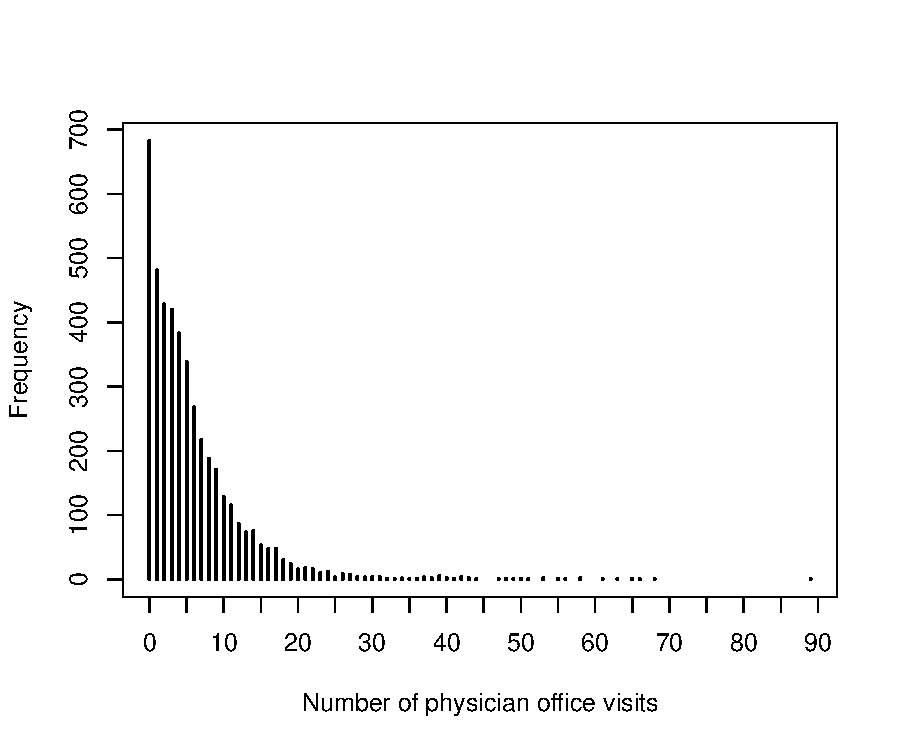
\includegraphics{countreg-ofp-plot2}
\caption{\label{fig:ofp} Frequency distribution for number of physician office visits.}
\end{center}
\end{figure}

\setkeys{Gin}{width=\textwidth} 
\begin{figure}[p]
\begin{center}
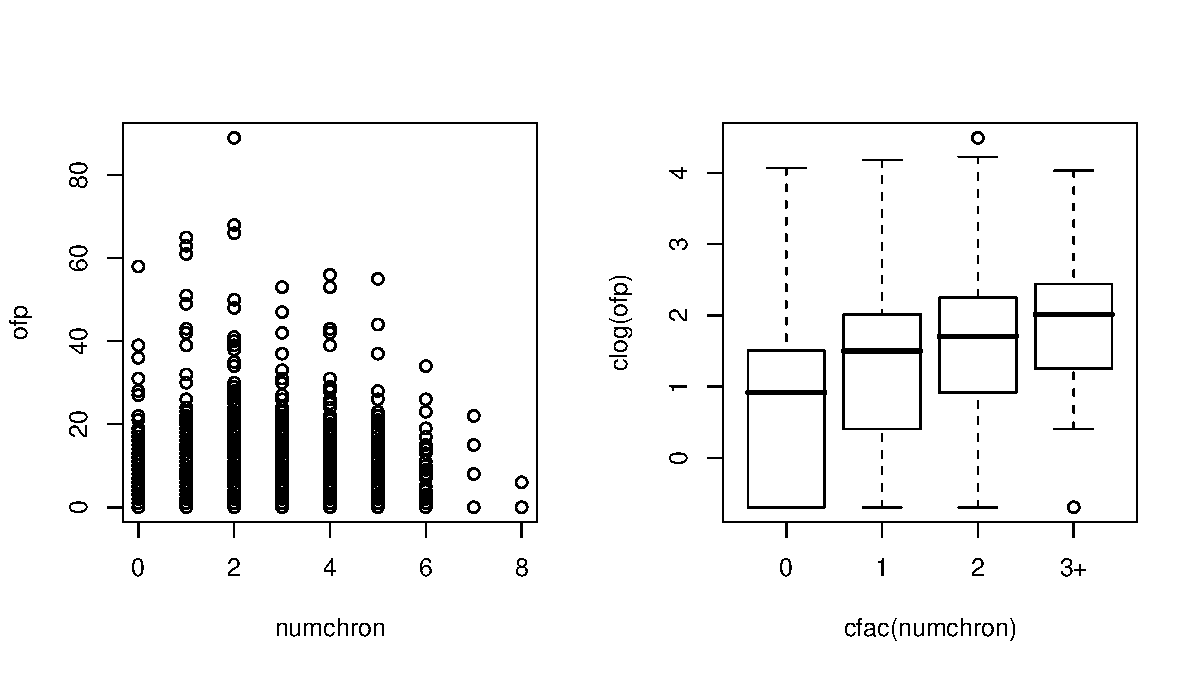
\includegraphics{countreg-bad-good}
\caption{\label{fig:bad-good} Bivariate explorative displays for number of physician office visits
  plotted against number of chronic conditions.}
\end{center}
\end{figure}

A natural second step in the exploratory analysis is to look at pairwise bivariate 
displays of the dependent variable against each of the regressors bringing out the
partial relationships. In \proglang{R}, such bivariate displays
can easily be generated with the \fct{plot} method for formulas, e.g., via \code{plot(y ~ x)}.
This chooses different types of displays depending on the combination of quantitative
and qualitative variables as dependent or regressor variable, respectively. However,
count variables are treated as all numerical variables and therefore the command

\begin{Schunk}
\begin{Sinput}
R> plot(ofp ~ numchron, data = dt)
\end{Sinput}
\end{Schunk}

produces a simple scatterplot as shown in the left panel of Figure~\ref{fig:bad-good}.
This is clearly not useful as both variables are count variables producing numerous
ties in the bivariate distribution and thus obscuring a large number of points in
the display. To overcome the problem, it is useful to group the number of chronic
conditions into a factor with levels `0', `1', `2', and `3 or more' and produce a
boxplot instead of a scatterplot. Furthermore, the picture is much clearer if the
dependent variable is log-transformed (just as all count regression models discussed
above also use a log link by default). As there are zero counts as well, we use a
convenience function \fct{clog} providing a continuity-corrected logarithm.

\begin{Schunk}
\begin{Sinput}
R> clog <- function(x) log(x + 0.5)
\end{Sinput}
\end{Schunk}

For transforming a count variable to a factor (for visualization purposes only),
we define another convenience function \fct{cfac}

\begin{Schunk}
\begin{Sinput}
R> cfac <- function(x, breaks = NULL) {
+   if(is.null(breaks)) breaks <- unique(quantile(x, 0:10/10))
+   x <- cut(x, breaks, include.lowest = TRUE, right = FALSE)
+   levels(x) <- paste(breaks[-length(breaks)], ifelse(diff(breaks) > 1,
+     c(paste("-", breaks[-c(1, length(breaks))] - 1, sep = ""), "+"), ""),
+     sep = "")
+   return(x)
+ }
\end{Sinput}
\end{Schunk}

which by default tries to take an educated guess how to choose the breaks between the categories.
Clearly, the resulting exploratory display of the transformed variables produced by

\begin{Schunk}
\begin{Sinput}
R> plot(clog(ofp) ~ cfac(numchron), data = dt)
\end{Sinput}
\end{Schunk}

(shown in the right panel of Figure~\ref{fig:bad-good}) brings out much better
how the number of doctor visits increases with the number of chronic conditions.

\setkeys{Gin}{width=\textwidth} 
\begin{figure}[p]
\begin{center}
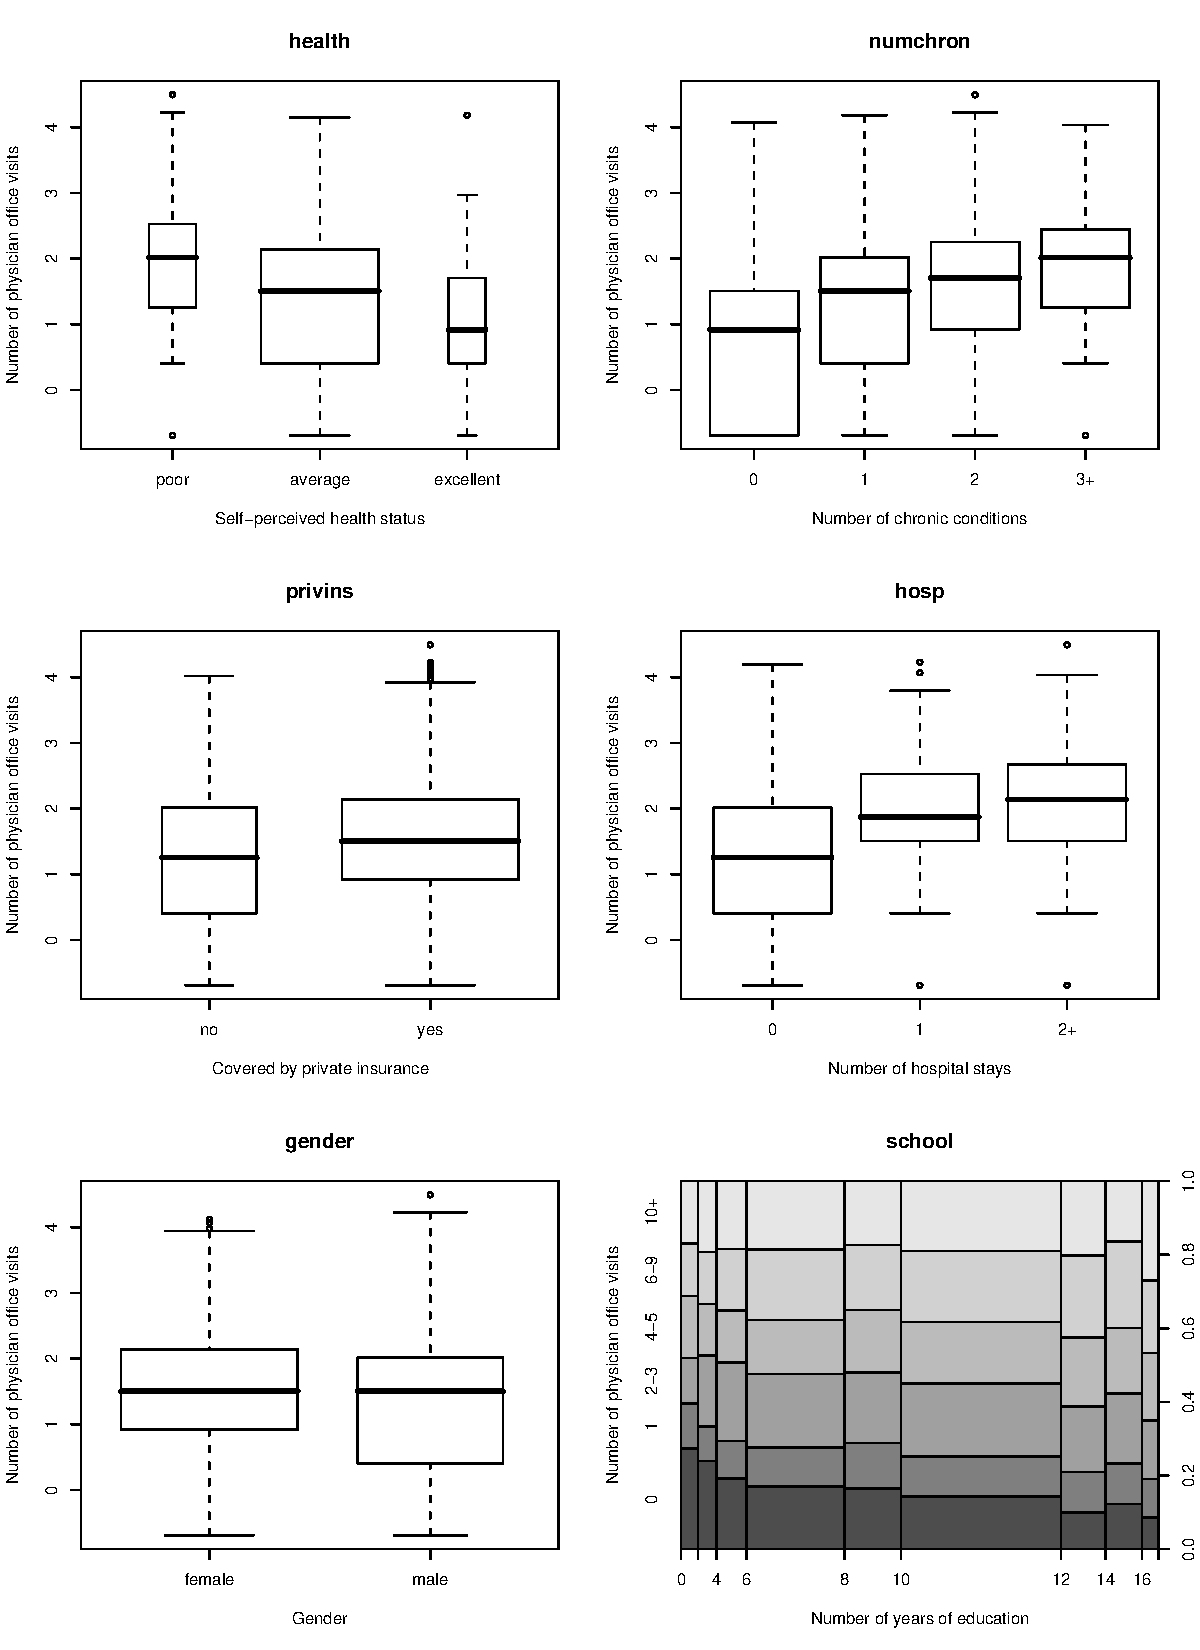
\includegraphics{countreg-ofp2-plot1}
\caption{\label{fig:ofp2} Number of physician office visits plotted against regressors used.}
\end{center}
\end{figure}

Analogous displays for the number of physician office visits against all regressors
can be produced via
\begin{Schunk}
\begin{Sinput}
R> plot(clog(ofp) ~ health, data = dt, varwidth = TRUE)
R> plot(clog(ofp) ~ cfac(numchron), data = dt)
R> plot(clog(ofp) ~ privins, data = dt, varwidth = TRUE)
R> plot(clog(ofp) ~ cfac(hosp, c(0:2, 8)), data = dt)
R> plot(clog(ofp) ~ gender, data = dt, varwidth = TRUE)
R> plot(cfac(ofp, c(0:2, 4, 6, 10, 100)) ~ school, data = dt, breaks = 9)
\end{Sinput}
\end{Schunk}
and are shown (with slightly enhanced labeling) in Figure~\ref{fig:ofp2}. 
The last plot uses a different type of display. Here, the dependent count variable
is not log-transformed but grouped into a factor and then a spinogram
is produced. This also groups the regressor (as in a histogram) and then
produces a highlighted mosaic plot. All displays show that the number of
doctor visits increases or decreases with the regressors as expected: \code{ofp}
decreases with the general health status but increases with the number of
chronic conditions or hospital stays. The average number of visits is also
slightly higher for patients with a private insurance and higher level of 
education. It is slightly lower for male compared to female patients.
The overall impression from all displays is that the changes in the mean
can only explain a modest amount of variation in the data.


\subsection{Poisson regression}

As a first attempt to capture the relationship between the number of 
physician office visits and all regressors---described in \proglang{R} by the
formula \code{ofp ~ .}---in a parametric
regression model, we fit the basic Poisson regression model
\begin{Schunk}
\begin{Sinput}
R> fm_pois <- glm(ofp ~ ., data = dt, family = poisson)
\end{Sinput}
\end{Schunk}
and obtain the coefficient estimates along with associated partial Wald tests
\begin{Schunk}
\begin{Sinput}
R> summary(fm_pois)
\end{Sinput}
\begin{Soutput}
Call:
glm(formula = ofp ~ ., family = poisson, data = dt)

Deviance Residuals: 
    Min       1Q   Median       3Q      Max  
-8.4055  -1.9962  -0.6737   0.7049  16.3620  

Coefficients:
                 Estimate Std. Error z value Pr(>|z|)    
(Intercept)      1.028874   0.023785  43.258   <2e-16 ***
hosp             0.164797   0.005997  27.478   <2e-16 ***
healthpoor       0.248307   0.017845  13.915   <2e-16 ***
healthexcellent -0.361993   0.030304 -11.945   <2e-16 ***
numchron         0.146639   0.004580  32.020   <2e-16 ***
gendermale      -0.112320   0.012945  -8.677   <2e-16 ***
school           0.026143   0.001843  14.182   <2e-16 ***
privinsyes       0.201687   0.016860  11.963   <2e-16 ***
---
Signif. codes:  0 ‘***’ 0.001 ‘**’ 0.01 ‘*’ 0.05 ‘.’ 0.1 ‘ ’ 1 

(Dispersion parameter for poisson family taken to be 1)

    Null deviance: 26943  on 4405  degrees of freedom
Residual deviance: 23168  on 4398  degrees of freedom
AIC: 35959

Number of Fisher Scoring iterations: 5
\end{Soutput}
\end{Schunk}
All coefficient estimates confirm the results from the exploratory analysis
in Figure~\ref{fig:ofp2}. All coefficients are highly significant with the
health variables leading to somewhat larger Wald statistics compared to the
socio-economic variables. However, the Wald test
results might be too optimistic due to a misspecification of the likelihood.
As the exploratory analysis suggested that over-dispersion is present in this data
set, we re-compute the Wald tests using sandwich standard errors
\begin{Schunk}
\begin{Sinput}
R> coeftest(fm_pois, vcov = sandwich)
\end{Sinput}
\begin{Soutput}
z test of coefficients:

                 Estimate Std. Error z value  Pr(>|z|)    
(Intercept)      1.028874   0.064530 15.9442 < 2.2e-16 ***
hosp             0.164797   0.021945  7.5095 5.935e-14 ***
healthpoor       0.248307   0.054022  4.5964 4.298e-06 ***
healthexcellent -0.361993   0.077449 -4.6740 2.954e-06 ***
numchron         0.146639   0.012908 11.3605 < 2.2e-16 ***
gendermale      -0.112320   0.035343 -3.1780  0.001483 ** 
school           0.026143   0.005084  5.1422 2.715e-07 ***
privinsyes       0.201687   0.043128  4.6765 2.919e-06 ***
---
Signif. codes:  0 ‘***’ 0.001 ‘**’ 0.01 ‘*’ 0.05 ‘.’ 0.1 ‘ ’ 1 
\end{Soutput}
\end{Schunk}
All regressors are still significant but the standard errors seem to be more
appropriate. This will also be confirmed by the following models that
deal with over-dispersion (and excess zeros) in a more formal way.

\subsection{Quasi-Poisson regression}

The quasi-Poisson model
\begin{Schunk}
\begin{Sinput}
R> fm_qpois <- glm(ofp ~ ., data = dt, family = quasipoisson)
\end{Sinput}
\end{Schunk}
leads to an estimated dispersion of
$\hat \phi = 6.706$ which
is clearly larger than $1$ confirming that over-dispersion is present in
the data.\footnote{Alternatively, over-dispersion can be confirmed by comparison
of the log-likelihoods of the Poisson and negative binomial model.}
The resulting partial Wald tests of the coefficients
are rather similar to the results obtained from the Poisson regression with
sandwich standard errors, leading to the same conclusions. As before, they
can be obtained via
\begin{Schunk}
\begin{Sinput}
R> summary(fm_qpois)
\end{Sinput}
\end{Schunk}
The output is suppressed here and is presented in tabular form in Table~\ref{tab:summary}.


\subsection{Negative binomial regression}

A more formal way to accommodate over-dispersion in a count data regression
model is to use a negative binomial model.
\begin{Schunk}
\begin{Sinput}
R> fm_nbin <- glm.nb(ofp ~ ., data = dt)
R> summary(fm_nbin)
\end{Sinput}
\end{Schunk}
As shown in Table~\ref{tab:summary},
both regression coefficients and standard errors are rather similar
to the quasi-Poisson and the sandwich-adjusted Poisson results above. Thus,
in terms of predicted means all three models give very similar results;
the associated partial Wald tests also lead to the same conclusions.

One advantage of the negative binomial model is that it is associated with a formal
likelihood so that information criteria are readily available. Furthermore, the expected
number of zeros can be computed from the fitted densities via 
$\sum_i f(0, \hat \mu_i, \hat \theta)$. 


\subsection{Hurdle regression}

The exploratory analysis conveyed the impression that there might be more zero observations
than explained by the basic count data distributions, hence a negative
binomial hurdle model is fitted via
\begin{Schunk}
\begin{Sinput}
R> fm_hurdle0 <- hurdle(ofp ~ ., data = dt, dist = "negbin")
\end{Sinput}
\end{Schunk}
This uses the same type of count data model as in the preceeding section
but it is now truncated for \code{ofp < 1} and has an additional hurdle
component modeling zero vs.\ count observations. By default, the hurdle
component is a binomial GLM with logit link which contains all regressors used in the count
model. The associated coefficient estimates and partial Wald tests for
both model components are displayed via
\begin{Schunk}
\begin{Sinput}
R> summary(fm_hurdle0)
\end{Sinput}
\begin{Soutput}
Call:
hurdle(formula = ofp ~ ., data = dt, dist = "negbin")


Count model coefficients (truncated negbin with log link):
                 Estimate Std. Error z value Pr(>|z|)    
(Intercept)      1.197699   0.058973  20.309  < 2e-16 ***
hosp             0.211898   0.021396   9.904  < 2e-16 ***
healthpoor       0.315958   0.048056   6.575 4.87e-11 ***
healthexcellent -0.331861   0.066093  -5.021 5.14e-07 ***
numchron         0.126421   0.012452  10.152  < 2e-16 ***
gendermale      -0.068317   0.032416  -2.108   0.0351 *  
school           0.020693   0.004535   4.563 5.04e-06 ***
privinsyes       0.100172   0.042619   2.350   0.0188 *  
Log(theta)       0.333255   0.042754   7.795 6.46e-15 ***
Zero hurdle model coefficients (binomial with logit link):
                 Estimate Std. Error z value Pr(>|z|)    
(Intercept)      0.043147   0.139852   0.309 0.757688    
hosp             0.312449   0.091437   3.417 0.000633 ***
healthpoor      -0.008716   0.161024  -0.054 0.956833    
healthexcellent -0.289570   0.142682  -2.029 0.042409 *  
numchron         0.535213   0.045378  11.794  < 2e-16 ***
gendermale      -0.415658   0.087608  -4.745 2.09e-06 ***
school           0.058541   0.011989   4.883 1.05e-06 ***
privinsyes       0.747120   0.100880   7.406 1.30e-13 ***
---
Signif. codes:  0 '***' 0.001 '**' 0.01 '*' 0.05 '.' 0.1 ' ' 1 

Theta: count = 1.3955
Number of iterations in BFGS optimization: 16 
Log-likelihood: -1.209e+04 on 17 Df
\end{Soutput}
\end{Schunk}
The coefficients in the count component resemble those from the previous
models, but the increase in the log-likelihood (see also Table~\ref{tab:summary})
conveys that the model has improved by including the hurdle component.
However, it might be possible to omit the \code{health} variable from
the hurdle model. To test this hypothesis, the reduced model is fitted
via
\begin{Schunk}
\begin{Sinput}
R> fm_hurdle <- hurdle(ofp ~ . | hosp + numchron + privins + school + gender,
+   data = dt, dist = "negbin")
\end{Sinput}
\end{Schunk}
and can then be compared to the full model in a Wald test
\begin{Schunk}
\begin{Sinput}
R> waldtest(fm_hurdle0, fm_hurdle)
\end{Sinput}
\begin{Soutput}
Wald test

Model 1: ofp ~ .
Model 2: ofp ~ . | hosp + numchron + privins + school + gender
  Res.Df   Df  Chisq Pr(>Chisq)
1   4389                       
2   4391   -2 4.1213     0.1274
\end{Soutput}
\end{Schunk}
or LR test
\begin{Schunk}
\begin{Sinput}
R> lrtest(fm_hurdle0, fm_hurdle)
\end{Sinput}
\end{Schunk}
which leads to virtually identical results.

\begin{table}[t!]
\begin{center}
\begin{tabular}{|l|rrrr|rr|} \hline
Type & \multicolumn{4}{|c|}{GLM} & \multicolumn{2}{|c|}{zero-augmented} \\
Distribution & \multicolumn{3}{|c}{Poisson} & \multicolumn{1}{c|}{NB} &
  \multicolumn{1}{|c}{Hurdle-NB} & \multicolumn{1}{c|}{ZINB} \\
Method & \multicolumn{1}{|c}{ML} & \multicolumn{1}{c}{adjusted} & \multicolumn{1}{c}{quasi} &
  \multicolumn{1}{c|}{ML} & \multicolumn{1}{|c}{ML} & \multicolumn{1}{c|}{ML} \\ 
Object & \code{fm_pois} & \code{fm_pois} & \code{fm_qpois} & \code{fm_nbin} & \code{fm_hurdle} & \code{fm_zinb} \\ \hline
\code{(Intercept)} & $ 1.029$\phantom{)} & $ 1.029$\phantom{)} & $ 1.029$\phantom{)} & $ 0.929$\phantom{)} & $ 1.198$\phantom{)} & $ 1.194$\phantom{)} \\
 & (0.024) & (0.065) & (0.062) & (0.055) & (0.059) & (0.057) \\
\code{hosp} & $ 0.165$\phantom{)} & $ 0.165$\phantom{)} & $ 0.165$\phantom{)} & $ 0.218$\phantom{)} & $ 0.212$\phantom{)} & $ 0.201$\phantom{)} \\
 & (0.006) & (0.022) & (0.016) & (0.020) & (0.021) & (0.020) \\
\code{healthpoor} & $ 0.248$\phantom{)} & $ 0.248$\phantom{)} & $ 0.248$\phantom{)} & $ 0.305$\phantom{)} & $ 0.316$\phantom{)} & $ 0.285$\phantom{)} \\
 & (0.018) & (0.054) & (0.046) & (0.049) & (0.048) & (0.045) \\
\code{healthexcellent} & $-0.362$\phantom{)} & $-0.362$\phantom{)} & $-0.362$\phantom{)} & $-0.342$\phantom{)} & $-0.332$\phantom{)} & $-0.319$\phantom{)} \\
 & (0.030) & (0.077) & (0.078) & (0.061) & (0.066) & (0.060) \\
\code{numchron} & $ 0.147$\phantom{)} & $ 0.147$\phantom{)} & $ 0.147$\phantom{)} & $ 0.175$\phantom{)} & $ 0.126$\phantom{)} & $ 0.129$\phantom{)} \\
 & (0.005) & (0.013) & (0.012) & (0.012) & (0.012) & (0.012) \\
\code{gendermale} & $-0.112$\phantom{)} & $-0.112$\phantom{)} & $-0.112$\phantom{)} & $-0.126$\phantom{)} & $-0.068$\phantom{)} & $-0.080$\phantom{)} \\
 & (0.013) & (0.035) & (0.034) & (0.031) & (0.032) & (0.031) \\
\code{school} & $ 0.026$\phantom{)} & $ 0.026$\phantom{)} & $ 0.026$\phantom{)} & $ 0.027$\phantom{)} & $ 0.021$\phantom{)} & $ 0.021$\phantom{)} \\
 & (0.002) & (0.005) & (0.005) & (0.004) & (0.005) & (0.004) \\
\code{privinsyes} & $ 0.202$\phantom{)} & $ 0.202$\phantom{)} & $ 0.202$\phantom{)} & $ 0.224$\phantom{)} & $ 0.100$\phantom{)} & $ 0.126$\phantom{)} \\
 & (0.017) & (0.043) & (0.044) & (0.039) & (0.043) & (0.042) \\ \hline
\code{(Intercept)} &   &   &   &   & $ 0.016$\phantom{)} & $-0.047$\phantom{)} \\
 &   &   &   &   & (0.138) & (0.269) \\
\code{hosp} &   &   &   &   & $ 0.318$\phantom{)} & $-0.800$\phantom{)} \\
 &   &   &   &   & (0.091) & (0.421) \\
\code{numchron} &   &   &   &   & $ 0.548$\phantom{)} & $-1.248$\phantom{)} \\
 &   &   &   &   & (0.044) & (0.178) \\
\code{privinsyes} &   &   &   &   & $ 0.746$\phantom{)} & $-1.176$\phantom{)} \\
 &   &   &   &   & (0.100) & (0.220) \\
\code{school} &   &   &   &   & $ 0.057$\phantom{)} & $-0.084$\phantom{)} \\
 &   &   &   &   & (0.012) & (0.026) \\
\code{gendermale} &   &   &   &   & $-0.419$\phantom{)} & $ 0.648$\phantom{)} \\
 &   &   &   &   & (0.088) & (0.200) \\ \hline
no.\ parameters & 8 & 8 & 8 & 9 & 15 & 15 \\
$\log L$ & -17971.6 &   &   & -12170.6 & -12090.1 & -12090.7 \\
AIC & 35959.2 &   &   & 24359.1 & 24210.1 & 24211.4 \\
BIC & 36010.4 &   &   & 24416.6 & 24306.0 & 24307.3 \\
$\sum_i \hat f_i(0)$ & 47 &   &   & 608 & 683 & 709 \\ \hline\end{tabular}
\caption{\label{tab:summary} Summary of fitted count regression models for NMES data:
 coefficient estimates from count model, zero-inflation model (both with standard errors
 in parantheses), number of estimated parameters, maximized log-likelihood, AIC, BIC
 and expected number of zeros (sum of fitted densities evaluated at zero). The observed
 number of zeros is 683 in 4406 observations.}
\end{center}
\end{table}


\subsection{Zero-inflated regression}

A different way of augmenting the negative binomial count model \code{fm_nbin}
with additional probability weight for zero counts is a zero-inflated
negative binomial (ZINB) regression. The default model is fitted via
\begin{Schunk}
\begin{Sinput}
R> fm_zinb0 <- zeroinfl(ofp ~ ., data = dt, dist = "negbin")
\end{Sinput}
\end{Schunk}
This has just an intercept in the zero-inflation model, but---as the hurdle
model \code{fm_hurdle} fitted above has shown---the available regressors can be
used for distinguishing between zero and larger counts. Therefore, a second
model is fitted
\begin{Schunk}
\begin{Sinput}
R> fm_zinb <- zeroinfl(ofp ~ . | hosp + numchron + privins + school + gender,
+   data = dt, dist = "negbin")
\end{Sinput}
\end{Schunk}
that has the same variables in the zero-inflation part as the hurdle
component in \code{fm_hurdle}. This improves the ZINB fit significantly
which can again be brought out by a Wald test
\begin{Schunk}
\begin{Sinput}
R> waldtest(fm_zinb0, fm_zinb)
\end{Sinput}
\begin{Soutput}
Wald test

Model 1: ofp ~ .
Model 2: ofp ~ . | hosp + numchron + privins + school + gender
  Res.Df   Df  Chisq Pr(>Chisq)    
1   4396                           
2   4391    5 115.72  < 2.2e-16 ***
---
Signif. codes:  0 ‘***’ 0.001 ‘**’ 0.01 ‘*’ 0.05 ‘.’ 0.1 ‘ ’ 1 
\end{Soutput}
\end{Schunk}
or a LR test \code{lrtest(fm_zinb0, fm_zinb)} that produces virtually identical
results. The chosen fitted model can again be inspected via
\begin{Schunk}
\begin{Sinput}
R> summary(fm_zinb)
\end{Sinput}
\end{Schunk}
See Table~\ref{tab:summary} for a more concise summary.

\subsection{Comparison}

Having fitted several count data regression models to the demand for medical care
in the NMES data, it is, of course, of interest to understand what these models have
in common and what their differences are. In this section, we show how to compute
the components of Table~\ref{tab:summary} and provide some further comments and
interpretations. 

As a first comparison, it is of natural
interest to inspect the estimated regression coefficients in the count data model

\begin{Schunk}
\begin{Sinput}
R> fm <- list("ML-Pois" = fm_pois, "Quasi-Pois" = fm_qpois, "NB" = fm_nbin,
+   "Hurdle-NB" = fm_hurdle, "ZINB" = fm_zinb)
R> round(sapply(fm, function(x) coef(x)[1:8]), digits = 3)
\end{Sinput}
\begin{Soutput}
                ML-Pois Quasi-Pois     NB Hurdle-NB   ZINB
(Intercept)       1.029      1.029  0.929     1.198  1.194
hosp              0.165      0.165  0.218     0.212  0.201
healthpoor        0.248      0.248  0.305     0.316  0.285
healthexcellent  -0.362     -0.362 -0.342    -0.332 -0.319
numchron          0.147      0.147  0.175     0.126  0.129
gendermale       -0.112     -0.112 -0.126    -0.068 -0.080
school            0.026      0.026  0.027     0.021  0.021
privinsyes        0.202      0.202  0.224     0.100  0.126
\end{Soutput}
\end{Schunk}

This shows that there are some small differences, especially between the GLMs and the
zero-augmented models. However, the zero-augmented models have to be interpreted 
slightly differently: While the GLMs all have the same mean function (\ref{eq:mean}),
the zero-augmentation also enters the mean function, see (\ref{eq:zeroinfl-mean}) and
(\ref{eq:hurdle-mean}). Nevertheless,
the overall impression is that the estimated mean functions are rather similar.
Moreover, the associated estimated standard errors
are very similar as well:
\begin{Schunk}
\begin{Sinput}
R> round(cbind("ML-Pois" = sqrt(diag(vcov(fm_pois))),
+   "Adj-Pois" = sqrt(diag(sandwich(fm_pois))),
+   sapply(fm[-1], function(x) sqrt(diag(vcov(x)))[1:8])),
+   digits = 3)
\end{Sinput}
\begin{Soutput}
                ML-Pois Adj-Pois Quasi-Pois    NB Hurdle-NB  ZINB
(Intercept)       0.024    0.065      0.062 0.055     0.059 0.057
hosp              0.006    0.022      0.016 0.020     0.021 0.020
healthpoor        0.018    0.054      0.046 0.049     0.048 0.045
healthexcellent   0.030    0.077      0.078 0.061     0.066 0.060
numchron          0.005    0.013      0.012 0.012     0.012 0.012
gendermale        0.013    0.035      0.034 0.031     0.032 0.031
school            0.002    0.005      0.005 0.004     0.005 0.004
privinsyes        0.017    0.043      0.044 0.039     0.043 0.042
\end{Soutput}
\end{Schunk}
The only exception are the model-based standard errors for the Poisson model,
when treated as a fully specified model, which is obviously not appropriate for this data set.

In summary, the models are not too different with respect to their fitted 
mean functions. The differences become obvious if not only the mean but the
full likelihood is considered:
\begin{Schunk}
\begin{Sinput}
R> rbind(logLik = sapply(fm, function(x) round(logLik(x), digits = 0)),
+   Df = sapply(fm, function(x) attr(logLik(x), "df")))
\end{Sinput}
\begin{Soutput}
       ML-Pois Quasi-Pois     NB Hurdle-NB   ZINB
logLik  -17972         NA -12171    -12090 -12091
Df           8          8      9        15     15
\end{Soutput}
\end{Schunk}
The ML Poisson model is clearly inferior to all other fits. The quasi-Poisson
model and the sandwich-adjusted Poisson model are not associated with a fitted
likelihood. The negative binomial already improves the fit dramatically but
can in turn be improved by the hurdle and zero-inflated models which give
almost identical fits. This also reflects that the over-dispersion in the data
is captured better by the negative-binomial-based models than the plain
Poisson model. Additionally, it is of interest how the zero counts
are captured by the various models. Therefore, the observed zero counts are
compared to expected number of zero counts for the likelihood based models:
\begin{Schunk}
\begin{Sinput}
R> round(c("Obs" = sum(dt$ofp < 1),
+   "ML-Pois" = sum(dpois(0, fitted(fm_pois))),
+   "Adj-Pois" = NA,
+   "Quasi-Pois" = NA,
+   "NB" = sum(dnbinom(0, mu = fitted(fm_nbin), size = fm_nbin$theta)),
+   "NB-Hurdle" = sum(predict(fm_hurdle, type = "prob")[,1]),
+   "ZINB" = sum(predict(fm_zinb, type = "prob")[,1])))
\end{Sinput}
\begin{Soutput}
       Obs    ML-Pois   Adj-Pois Quasi-Pois         NB  NB-Hurdle       ZINB 
       683         47         NA         NA        608        683        709 
\end{Soutput}
\end{Schunk}
Thus, the ML Poisson model is again not appropriate whereas the negative-binomial-based
models are much better in modeling the zero counts. By construction, the
expected number of zero counts in the hurdle model matches the observed
number.

In summary, the hurdle and zero-inflation models lead to the best 
results (in terms of likelihood) on this data set. Above, their mean function for the
count component was already shown to be very similar, below we take a
look at the fitted zero components:
\begin{Schunk}
\begin{Sinput}
R> t(sapply(fm[4:5], function(x) round(x$coefficients$zero, digits = 3)))
\end{Sinput}
\begin{Soutput}
          (Intercept)   hosp numchron privinsyes school gendermale
Hurdle-NB       0.016  0.318    0.548      0.746  0.057     -0.419
ZINB           -0.047 -0.800   -1.248     -1.176 -0.084      0.648
\end{Soutput}
\end{Schunk}
This shows that the absolute values are rather different---which is not
surprising as they pertain to slightly different ways of modeling zero
counts---but the signs of the coefficients match, i.e., are just inversed.
For the hurdle model, the zero hurdle component describes the probability
of observing a positive count whereas, for the ZINB model, the zero-inflation
component predicts the probability of observing a zero count from the
point mass component. Overall, both models lead to the same qualitative
results and very similar model fits. Perhaps, the hurdle model is slightly
preferable because it has the nicer interpretation: there is one process
that controls whether a patient sees a physician or not, and a second 
process that determines how many office visits are made.

\section{Summary} \label{sec:summary}

The model frame for basic count data models from the GLM framework as well
as their implementation in the \proglang{R} system for statistical computing
is reviewed. Starting from these basic tools, it is presented how
zero-inflated and hurdle models extend the classical models and how
likewise their \proglang{R} implementation in package \pkg{pscl} re-uses
design and functionality of the corresponding \proglang{R} software.
Hence, the new functions \fct{zeroinfl} and \fct{hurdle} are straightforward
to apply for model fitting. Additionally, standard methods for diagnostics 
are provided and generic inference tools from other packages can easily be
re-used.


\section*{Computational details}

The results in this paper were obtained using
\proglang{R}~2.7.0 with the packages
\pkg{MASS}~7.2--40,
\pkg{pscl}~0.94,
\pkg{sandwich}~2.1--0,
\pkg{car}~1.2--7,
\pkg{lmtest}~0.9--21.
\proglang{R} itself and all packages used are available from
CRAN at \url{http://CRAN.R-project.org/}.

\bibliography{countreg}

\newpage

\begin{appendix}

\section{Technical details for zero-inflated models} \label{app:zeroinfl}

The fitting of zero-inflated models via ML in \fct{zeroinfl} is controlled by
the arguments in the \fct{zeroinfl.control} wrapper function:

\begin{Soutput}
zeroinfl.control(method = "BFGS", maxit = 10000, trace = FALSE,
  EM = FALSE, start = NULL, ...)
\end{Soutput}

This modifies some default arguments passed on to the optimizer \fct{optim},
such as \code{method}, \code{maxit} and \code{trace}. The latter is also
used within \fct{zeroinfl} and can be set to produce more verbose output
concerning the fitting process. The arguments \code{EM} and \code{start}
control the choice of starting values for calling \fct{optim}, all remaining
arguments passed through \code{...} are directly passed on to \fct{optim}.

By default, starting values are estimated by calling \fct{glm.fit} for
both components of the model separately, once for the counts and once
for zero vs.\ non-zero counts.
If \code{EM = TRUE}, this process is iterated until convergence of the
parameters to the ML estimates. The optimizer is still called subsequently
for a single iteration to obtain the Hessian matrix from which the estimated
covariance matrix can be computed. If starting values are supplied,
\code{start} needs to be set to a named list with the parameters for the
\code{$count} and \code{$zero} part of the model (and potentially a
\code{$theta} dispersion parameter if a negative binomial distribution is used).

The fitted model object of class \class{zeroinfl} is similar to \class{glm}
objects and contains sufficient information on all aspects of the fitting
process. In particular, the estimated parameters and associated covariances
are included as well as the result from the \fct{optim} call. Furthermore,
the call, formula, terms structure etc.\ is contained, potentially also the
model frame, dependent variable and regressor matrices.

Following \fct{glm.nb}, the $\theta$ parameter of the negative binomial
distribution is treated as a nuisance parameter. Thus, the \code{$coefficients}
component of the fitted model object just contains estimates of
$\beta$ and $\gamma$ while the estimate of $\theta$ and its standard deviation 
(on a log scale) are kept in extra list elements \code{$theta} and \code{$SE.logtheta}.


\section{Technical details for hurdle models} \label{app:hurdle}

Both the interface of the \fct{hurdle} function as well as its fitted
model objects are virtually identical to the corresponding \class{zeroinfl}
functionality. Hence, we only provide some additional information for
those aspects that differ from those discussed above. The details of the
ML optimization are again provided by a \fct{hurdle.control} wrapper:

\begin{Soutput}
hurdle.control(method = "BFGS", maxit = 10000, trace = FALSE,
  separate = TRUE, start = NULL, ...)
\end{Soutput}

The only new argument here is the argument \code{separate} which controls
whether the two components of the model are optimized separately (the default)
or not. This is possible because there are no mixed sources for the zeros
in the data (unlike in zero-inflation models).

\section{Methods for fitted zero-inflated and hurdle models} \label{app:methods}

Users typically should not need to compute on the internal structure of
\class{zeroinfl} or \class{hurdle} objects because a set of standard extractor functions is provided,
an overview is given in Table~\ref{tab:methods}.
This includes methods to the generic functions \fct{print} and \fct{summary} which
print the estimated coefficients along with further information. The \fct{summary} in particular
supplies partial Wald tests based on the coefficients and the covariance matrix.
As usual, the \fct{summary} method returns an object of class \class{summary.zeroinfl}
or \class{summary.hurdle}, respectively, containing the relevant summary statistics
which can subsequently be printed using the associated \fct{print} method.

The methods for \fct{coef} and \fct{vcov} by default
return a single vector of coefficients and their associated covariance matrix,
respectively, i.e., all coefficients are concatenated. By setting their \code{model}
argument, the estimates for a single component only can be extracted. Concatenating
the parameters by default and providing a matching covariance matrix estimate
(that does not contain the covariances of further nuisance parameters) facilitates
the application of generic inference functions such as \fct{coeftest}, \fct{waldtest},
and \fct{linear.hypothesis}. All of these compute Wald tests for which coefficient
estimates and associated covariances is essentially all information required and 
can therefore be queried in an object-oriented way with the \fct{coef} and \fct{vcov}
methods.

Similarly, the \fct{terms} and \fct{model.matrix} extractors can
be used to extract the relevant information for either component of the model.
A \fct{logLik} method is provided, hence \fct{AIC}
can be called to compute information criteria and \fct{lrtest} for conducting
LR tests of nested models.

The \fct{predict} method computes predicted means (default) or probabilities (i.e.,
likelihood contributions) for observed or new data.\footnote{Additionally, the means
from the count and zero component, respectively, can be predicted. For the
count component, this is the predicted count mean (without inflation/hurdle).
For the zero component, this is the probability
of observing a zero from the point mass component in zero-inflated models
and the ratio of probabilities of observing non-zero counts in hurdle models.}
Predicted means for the observed data can also be obtained by the \fct{fitted} method. Deviations
between observed counts $y_i$ and predicted means $\hat \mu_i$ can be obtained
by the \fct{residuals} method returning either raw residuals $y_i - \hat \mu_i$
or the scaled Pearson residuals (raw residuals divided by square root of variance function)
with the latter being the default.

\begin{table}[t!]
\begin{center}
\begin{tabular}{|l|p{8.7cm}|}
\hline
Function & Description \\ \hline
\fct{print} & simple printed display with coefficient estimates\\
\fct{summary} & standard regression output (coefficient estimates, standard errors, partial Wald tests);
                returns an object of class ``\code{summary.}\textit{class}''
                containing the relevant summary statistics (which has a \fct{print} method) \\ 	\hline
\fct{coef} & extract coefficients of model (full or components), a single vector of all coefficients by default \\
\fct{vcov} & associated covariance matrix (with matching names) \\
\fct{predict} & predictions (means or probabilities) for new data \\
\fct{fitted} & fitted means for observed data \\
\fct{residuals} & extract residuals (raw response or Pearson) \\ \hline
\fct{terms} & extract terms of model components \\
\fct{model.matrix} & extract model matrix of model components \\
\fct{logLik} & extract fitted log-likelihood \\ \hline
\fct{coeftest} & partial Wald tests of coefficients \\
\fct{waldtest} & Wald tests of nested models \\
\fct{linear.hypothesis} & Wald tests of linear hypotheses \\
\fct{lrtest} & likelihood ratio tests of nested models \\
\fct{AIC} & compute information criteria (AIC, BIC, \dots) \\ \hline
\end{tabular}
\caption{\label{tab:methods} Functions and methods for objects of class \class{zeroinfl}
  and \class{hurdle}. The first three blocks refer to methods, the last block contains generic
  functions whose default methods work because of the information supplied by the methods above.}
\end{center}
\end{table}

\section{Replication of textbook results} \label{app:replication}

\citet[p.~204]{countreg:Cameron+Trivedi:1998} use a somewhat extended version
of the model employed above. Because not all variables in that extended
model are significant, a reduced set of variables was used throughout the main
paper. Here, however, we use the full model to show that the tools in \pkg{pscl}
reproduce the results of \cite{countreg:Cameron+Trivedi:1998}.

After omitting the responses other than \code{ofp} and setting \code{"other"}
as the reference category for \code{region}
\begin{Schunk}
\begin{Sinput}
R> dt2 <- DebTrivedi[, -(2:6)]
R> dt2$region <- relevel(dt2$region, "other")
\end{Sinput}
\end{Schunk}
we fit a model that contains all explanatory variables, both in the
count model and the zero hurdle model:
\begin{Schunk}
\begin{Sinput}
R> fm_hurdle2 <- hurdle(ofp ~ ., data = dt2, dist = "negbin")
\end{Sinput}
\end{Schunk}

The resulting coefficient estimates are virtually identical to those published
in \citet[p.~204]{countreg:Cameron+Trivedi:1998}. The associated Wald statistics
are also very similar provided that sandwich standard errors are used
\citet[which is not stated explicitely in][]{countreg:Cameron+Trivedi:1998}.
\begin{Schunk}
\begin{Sinput}
R> cfz <- coef(fm_hurdle2, model = "zero")
R> cfc <- coef(fm_hurdle2, model = "count")
R> se <- sqrt(diag(sandwich(fm_hurdle2)))
R> round(cbind(zero = cfz, zero_t = cfz/se[-seq(along = cfc)], 
+   count = cfc, count_t = cfc/se[seq(along = cfc)]),
+   digits = 3)[c(3, 2, 4, 5, 7, 6, 8, 9:17, 1),]
\end{Sinput}
\begin{Soutput}
                  zero zero_t  count count_t
healthexcellent -0.329 -2.310 -0.378  -4.312
healthpoor       0.071  0.420  0.333   5.863
numchron         0.557 10.547  0.143  10.520
adldiffyes      -0.188 -1.448  0.129   2.504
regionnoreast    0.129  1.033  0.104   1.974
regionmidwest    0.101  0.880 -0.016  -0.344
regionwest       0.202  1.509  0.123   2.444
age              0.190  2.348 -0.075  -2.339
blackyes        -0.327 -2.450  0.002   0.023
gendermale      -0.464 -4.715  0.004   0.098
marriedyes       0.247  2.379 -0.092  -2.110
school           0.054  4.109  0.022   3.824
faminc           0.007  0.365 -0.002  -0.380
employedyes     -0.012 -0.085  0.030   0.401
privinsyes       0.762  6.501  0.227   4.007
medicaidyes      0.554  3.055  0.185   2.777
(Intercept)     -1.475 -2.283  1.631   6.017
\end{Soutput}
\begin{Sinput}
R> logLik(fm_hurdle2)
\end{Sinput}
\begin{Soutput}
'log Lik.' -12110.49 (df=35)
\end{Soutput}
\begin{Sinput}
R> 1/fm_hurdle2$theta
\end{Sinput}
\begin{Soutput}
    count 
0.7437966 
\end{Soutput}
\end{Schunk}
There are some small and very few larger deviations in the Wald statistics
which are probably explicable by different approximations to the gradient
of $\theta$ (or $1/\theta$ or $\log(\theta)$) and the usage of different
non-linear optimizers (and at least ten years of software development).

\end{appendix}

\end{document}

%% Overdispersion tests
%% -> currently left out of the vignette until fixed and unified

\section{Technical documentation for dispersion tests}

The function \fct{dispersiontest} tests the null hypothesis of
equidispersion in Poisson GLMs against the alternative of overdispersion
and/or underdispersion.

\begin{Soutput}
dispersiontest(object, trafo = NULL, alternative = "greater")
\end{Soutput}

\begin{description}
  \item[\code{object}] a fitted Poisson GLM of class \class{glm} as fitted
    by \fct{glm} with family \fct{poisson}.
  \item[\code{trafo}] a specification of the alternative (see also below),
    can be numeric or a (positive) function or \code{NULL} (the default).
  \item[\code{alternative}] a character string specifying the alternative hypothesis:
    \code{"greater"} corresponds to overdispersion, \code{"less"} to
    underdispersion and \code{"two.sided"} to either one.
\end{description}

The standard Poisson GLM models the (conditional) mean
\eqn{\mathsf{E}[y] = \mu}{E[y] = mu} which is assumed to be equal to the
variance \eqn{\mathsf{VAR}[y] = \mu}{VAR[y] = mu}.

\fct{dispersiontest} assesses the hypothesis that this assumption holds (equidispersion) against
the alternative that the variance is of the form:

\begin{equation}
  \VAR[y_i \, | \, x_i] \quad = \quad \mu \; + \; \alpha \cdot \mathrm{trafo}(\mu).
\end{equation}

Overdispersion corresponds to $\alpha > 0$ and underdispersion to
$\alpha < 0$. The coefficient $\alpha$ can be estimated by an auxiliary OLS
regression and tested with the corresponding $t$ (or $z$) statistic
which is asymptotically standard normal under the null hypothesis.

Common specifications of the transformation function $\mathrm{trafo(\cdot)$ are
$\mathrm{trafo}(\mu) = \mu^2$ or $\mathrm{trafo}(\mu) = \mu$.
The former corresponds to a negative binomial model with quadratic variance function
(called NB2 by Cameron and Trivedi, 2005), the latter to a negative binomial
model with linear variance function (called NB1 by Cameron and Trivedi, 2005)
or quasi-Poisson model with dispersion parameter, i.e.,

\begin{equation}
  \VAR[y_i \, | \, x_i] \quad = \quad \phi \cdot \mu \; = \; (1 + \alpha) \cdot \mu.
\end{equation}

By default, for \code{trafo = NULL}, the latter dispersion formulation is used in
\fct{dispersiontest}. Otherwise, if \code{trafo} is specified, the test is formulated
in terms of the parameter $\alpha$. The transformation \code{trafo} can either
be specified as a function or an integer corresponding to the function
\verb/function(x) x^trafo/,
such that \code{trafo = 1} and \code{trafo = 2} yield the linear and quadratic formulations
respectively.

